\documentclass[a4paper]{article}
\usepackage{geometry}
\usepackage{graphicx}
\usepackage{natbib}
\usepackage{amsmath}
\usepackage{amssymb}
\usepackage{amsthm}
\usepackage{paralist}
\usepackage{epstopdf}
\usepackage{tabularx}
\usepackage{longtable}
\usepackage{multirow}
\usepackage{multicol}
\usepackage[hidelinks]{hyperref}
\usepackage{fancyvrb}
\usepackage{algorithm}
\usepackage{algorithmic}
\usepackage{float}
\usepackage{paralist}
\usepackage[svgname]{xcolor}
\usepackage{enumerate}
\usepackage{array}
\usepackage{times}
\usepackage{url}
\usepackage{fancyhdr}
\usepackage{comment}
\usepackage{environ}
\usepackage{times}
\usepackage{textcomp}
\usepackage{caption}


\urlstyle{rm}

\setlength\parindent{0pt} % Removes all indentation from paragraphs
\theoremstyle{definition}
\newtheorem{definition}{Definition}[]
\newtheorem{conjecture}{Conjecture}[]
\newtheorem{example}{Example}[]
\newtheorem{theorem}{Theorem}[]
\newtheorem{lemma}{Lemma}
\newtheorem{proposition}{Proposition}
\newtheorem{corollary}{Corollary}

\floatname{algorithm}{Procedure}
\renewcommand{\algorithmicrequire}{\textbf{Input:}}
\renewcommand{\algorithmicensure}{\textbf{Output:}}
\newcommand{\abs}[1]{\lvert#1\rvert}
\newcommand{\norm}[1]{\lVert#1\rVert}
\newcommand{\RR}{\mathbb{R}}
\newcommand{\CC}{\mathbb{C}}
\newcommand{\Nat}{\mathbb{N}}
\newcommand{\br}[1]{\{#1\}}
\DeclareMathOperator*{\argmin}{arg\,min}
\DeclareMathOperator*{\argmax}{arg\,max}
\renewcommand{\qedsymbol}{$\blacksquare$}

\definecolor{dkgreen}{rgb}{0,0.6,0}
\definecolor{gray}{rgb}{0.5,0.5,0.5}
\definecolor{mauve}{rgb}{0.58,0,0.82}

\newcommand{\Var}{\mathrm{Var}}
\newcommand{\Cov}{\mathrm{Cov}}

\newcommand{\vc}[1]{\boldsymbol{#1}}
\newcommand{\xv}{\vc{x}}
\newcommand{\Sigmav}{\vc{\Sigma}}
\newcommand{\alphav}{\vc{\alpha}}
\newcommand{\muv}{\vc{\mu}}

\newcommand{\red}[1]{\textcolor{red}{#1}}

\def\x{\mathbf x}
\def\y{\mathbf y}
\def\w{\mathbf w}
\def\v{\mathbf v}
\def\E{\mathbb E}
\def\V{\mathbb V}

% TO SHOW SOLUTIONS, include following (else comment out):
\newenvironment{soln}{
    \leavevmode\color{blue}\ignorespaces
}{}


\hypersetup{
%    colorlinks,
    linkcolor={red!50!black},
    citecolor={blue!50!black},
    urlcolor={blue!80!black}
}

\geometry{
  top=1in,            % <-- you want to adjust this
  inner=1in,
  outer=1in,
  bottom=1in,
  headheight=3em,       % <-- and this
  headsep=2em,          % <-- and this
  footskip=3em,
}


\pagestyle{fancyplain}
\lhead{\fancyplain{}{Homework 3}}
\rhead{\fancyplain{}{CS 760 Machine Learning}}
\cfoot{\thepage}

\title{\textsc{Homework 3}} % Title

%%% NOTE:  Replace 'NAME HERE' etc., and delete any "\red{}" wrappers (so it won't show up as red)

\author{
\red{$$DEEPAN DAS$$} \\
\red{$$ddas27$$}\\
} 

\date{}

\begin{document}

\maketitle 


\textbf{Instructions:} 
Although this is a programming homework, you only need to hand in a pdf answer file.
There is no need to submit the latex source or any code.
You can choose any programming language, as long as you implement the algorithm from scratch. 

Use this latex file as a template to develop your homework.
Submit your homework on time as a single pdf file to Canvas.
Please check Piazza for updates about the homework.

\section{A Simplified 1NN Classifier}
You are to implement a 1-nearest-neighbor learner for classification.
To simplify your work, your program can assume that
\begin{itemize}
\item each item has $d$ continuous features $\x \in \RR^d$
\item binary classification and the class label is encoded as $y \in \{0,1\}$
\item data files are in plaintext with one labeled item per line, separated by whitespace:
$$x_{11} \quad \ldots \quad x_{1d} \quad y_1$$
$$...$$
$$x_{n1} \quad \ldots \quad x_{nd} \quad y_n$$
\end{itemize}

Your program should implement a 1NN classifier: 
\begin{itemize}
\item Use Mahalanobis distance $d_A$ parametrized by a positive semidefinite (PSD) diagonal matrix $A$.  For $\x, \x' \in \RR^d$,
$$d_A(\x,\x') = \|\x-\x'\|_A = \sqrt{(\x-x')^\top A (\x-x')}.$$
We will specify $A$ in the questions below. (Hint: $d$ is dimension while $d_A$ with a subscript is distance)
\item If multiple training points are the equidistant nearest neighbors of a test point, you may use any one of those training points to predict the label.
\item You do not have to implement kd-tree.
\end{itemize}

\section{Questions}
\begin{enumerate}

\item (5 pts) What is the mathematical condition on the diagonal elements for a diagonal matrix $A$ to be PSD?

\begin{soln}

A matrix M is PSD for the following condition:

$$
A \hspace{0.3cm} PSD \Leftrightarrow  x^TAx \geq 0 \hspace{0.3cm} \forall x \in \mathbb{R}^n
$$
Thus, if $A \in \mathbb{R}^{dxd}$ and its diagonal elements are ${a_1, a_2, ..., a_d}$ , and let $x \in \mathbb{R}^d$ be defined as $[x_1, x_2, ... , x_d]$. Thus, $x^TAx \geq 0$ evaluates to:

$$x_1^2a_1 + x_2^2a_2 + ... + x_d^2a_d \geq 0$$

\textbf{Thus, we see, that all diagonal elements $\{a_1, a_2, ..., a_d\}$ should be greater than equal to zero}. Or, for every $a_i$ in $\{a_1, a_2, ..., a_d\}$, $a_i \geq 0$
\end{soln}

\item (5 pts) Given a training data set $D$, how do we preprocess it to make each feature dimension mean 0 and variance 1? (Hint: give the formula for $\hat \mu_j, \hat \sigma_j$ for each dimension $j$, and explain how to use them to normalize the data.  You may use either the $1 \over n$ or $1 \over n-1$ version of sample variance.  You may assume the sample variances are non-zero.) 


\begin{soln}
	Let $x_j$ be a feature in the dataset, where $x_j = [x_{1j}, x_{2j}, ... , x_{nj}]$. Then, the following operation can be applied to all the $x_{ij}$ in $x_j$ so as to make $x_j$ a feature $\tilde x_j$ with zero mean and unit variance.
	$$
	\tilde{x}_{i,j} = \frac{x_{i,j} - \hat \mu_{j}}{\hat \sigma_j} \hspace{0.3cm} \forall x_{ij} \in [x_{1j}, x_{2j}, ... , x_{nj}]$$
	Where, $\hat \mu_{j}$ refers to the mean across that $j$-th feature, and $\hat \sigma_j$ refers to the standard deviation
	$$
	\hat \mu_{j} = \frac{1}{n}\sum_{i=1}^{n} x_{ij}
	$$
	$$
	\hat \sigma_j = \sqrt{\frac{1}{n} \sum_{i=1}^{n} (x_{ij} - \hat \mu_{j})^2}
	$$
\end{soln}

\item (5 pts) Let $\tilde \x$ be the preprocessed data. Give the formula for the Euclidean distance between $\tilde \x, \tilde \x'$.

\begin{soln}
	The Euclidian distance can be expressed as :
	
	$$
	dist_{Euclidian}(\tilde x, \tilde x') = \sqrt{ \sum_{i=1}^{d} (\tilde x_{i} - \tilde x_{i}')^2} = \sqrt{(\tilde x-\tilde x')^\top I (\tilde x-\tilde x')} 
	$$
%	Thus,
%	
%	$$
%	dist_{Euclidian}(\tilde x, \tilde x') = || \tilde x - \tilde x'||_{A = I}
%	$$
%	where $A = I$, the Identity Matrix.
	
\end{soln}

\item (5 pts) Give the equivalent Mahalanobis distance on the original data $\x, \x'$ by specifying $A$. (Hint: you may need $\hat \mu_j, \hat \sigma_j$)

\begin{soln}
	Beginning from the Euclidian distance on the preprocessed data, we see that it can be written as:
	$$
	dist_{Euclidian}(\tilde x, \tilde x') = \sqrt{(\tilde x-\tilde x')^\top I (\tilde x-\tilde x')} 
	$$
	Now, $$\tilde x - \tilde x'  = [ (\frac{x_1 - \hat \mu_1}{\hat \sigma_1}  - \frac{x'_1 - \hat \mu_1}{\hat \sigma_1}), (\frac{x_2 - \hat \mu_2}{\hat \sigma_2}  - \frac{x'_2 - \hat \mu_2}{\hat \sigma_2}), ... , (\frac{x_d - \hat \mu_d}{\hat \sigma_d}  - \frac{x'_d - \hat \mu_d}{\hat \sigma_d}) ] = [\frac{(x_1 - x'_1 )}{\hat \sigma_1}, ..., \frac{(x_d - x'_d )}{\hat \sigma_d}] \in \mathbb{R}^d $$
	
	
%	In the Mahalanobis distance formulation as expressed above, $A$ can be specified as $S^{-1}$ where $S$ is the covariance matrix. Since it has been specified that $A$ is a diagonal matrix, $S$ is also a diagonal matrix with diagonal elements comprising of the variance in each feature. So, if we can define variance of the $j$-th feature as $\hat \sigma_j^2$, where, $	\hat \sigma_j^2 = \frac{1}{n} \sum_{i=1}^{n} (x_{ij} - \hat \mu_{j})^2
%	$, then, $A \in \mathbb{R}^{d \x d}$ can be defined as: 
Thus, 
	$$
	\sqrt{(\tilde x-\tilde x')^\top I (\tilde x-\tilde x')} = 
	\sqrt{(\x - \x')^\top
	\begin{pmatrix}
		\frac{1}{\hat \sigma_1^2} \hspace{0.3cm}0 \hspace{0.3cm} ...\hspace{0.3cm}0 \\
		0\hspace{0.3cm} \frac{1}{\hat \sigma_2^2} \hspace{0.3cm} ...\hspace{0.3cm}0 \\
		0\hspace{0.3cm} 0 \hspace{0.3cm} ... \hspace{0.3cm} \frac{1}{\hat \sigma_d^2} 
	\end{pmatrix}(\x - \x')}
	$$
	Thus, if we specify $A = \begin{pmatrix}
	\frac{1}{\hat \sigma_1^2} \hspace{0.3cm}0 \hspace{0.3cm} ...\hspace{0.3cm}0 \\
	0\hspace{0.3cm} \frac{1}{\hat \sigma_2^2} \hspace{0.3cm} ...\hspace{0.3cm}0 \\
	0\hspace{0.3cm} 0 \hspace{0.3cm} ... \hspace{0.3cm} \frac{1}{\hat \sigma_d^2} 
	\end{pmatrix}$,
	We can say that the following holds:
	$$
	\sqrt{(\tilde x-\tilde x')^\top I (\tilde x-\tilde x')} = \sqrt{(\x - \x')^\top A (\x - \x')} = d_A(\x,\x')
	$$
	
%	Now, replacing $A$ in the Mahalanobis distance formulation, we see,
%	
%	$$
%	d_A(\x,\x') = \|\x-\x'\|_A = \sqrt{(\x-x')^\top A (\x-x')} = \sqrt{ \sum_{i=1}^{d} \frac{(x_{i} - x_{i}')^2}{\hat \sigma_j^2}}
%	$$
	
\end{soln}

\item (5 pts) Let the diagonal elements of $A$ be $a_{11}, \ldots, a_{dd}$.
Define a diagonal matrix $L$ with diagonal $\sqrt{a_{11}}, \ldots, \sqrt{a_{dd}}$.
Define $\tilde \x = L\x$.
Prove that $d_I(\tilde \x, \tilde \x') = d_A(\x, \x')$ where $I$ is the identity matrix.

\begin{soln}
	We notice that $L^\top L = A$. So, 
	$$ 
	d_I(\tilde \x, \tilde \x') = \sqrt{(\tilde \x - \tilde \x')^\top I (\tilde \x- \tilde \x')} = 
	\sqrt{(L \x - L \x')^\top I (L \x- L\x')} = \sqrt{(\x - \x')^\top L^\top I L (\x- \x')}
	$$
	As, $L^\top I L = L^\top L = A$.
	Thus, 
	$$
    d_I(\tilde \x, \tilde \x') =  \sqrt{(\x - \x')^\top L^\top I L (\x- \x')} = \sqrt{(\x - \x')^\top A (\x- \x')} = d_A(\x, \x') 
    $$ 

%	= \sqrt{ \begin{pmatrix}  	\sqrt{a_{11}}x_1, \sqrt{a_{22}}x_2, ... ,\sqrt{a_{dd}}x_d \end{pmatrix} I  \begin{pmatrix}  	\sqrt{a_{11}}x_1 \\ \sqrt{a_{22}}x_2 \\ ... \\	\sqrt{a_{dd}}x_d \end{pmatrix} } = \sqrt{ \sum_{i=1}^{d} a_{ii} x_i^2} = \sqrt{ \begin{pmatrix}  	x_1, x_2, ... ,x_d \end{pmatrix} A \begin{pmatrix} 	x_1 \\ x_2 \\ ... \\	x_d \end{pmatrix} } = d_A(\x, \x')
%	$$
%	
\end{soln}

\item (5 pts) Geometrically, what does $L\x$ do to the point $\x$?  Explain in simple English.

\begin{soln}
	Essentially, since $L$ is a diagonal matrix, it applies a scaling on the $i$-th component of the data proportional to $\sqrt{a_{ii}}$. So each component gets scaled accordingly, and it produces a linear transformation geometrically, where each of the $d$-dimensions. This is essentially equal to a Hadamard product of the vectors $\{a_{11}, ... ,a_{dd}\}$ and $\{x_1, ... , x_d\}$. Each of the $x_i$'s get scaled and thus, transformed linearly. If all $a_{ii}$'s were equal, the transformation would be a linear scalar transformation, and it would be as if the magnitude of the vector $x$ was scaled by $a$ in the $d$-dimensional vector space.
\end{soln}
\item (10 pts) Let $U$ be any orthogonal matrix.
Define $\tilde \x = UL\x$.
(i) Prove that $d_I(\tilde \x, \tilde \x') = d_A(\x, \x')$ again. 
(ii) Geometrically, what does $UL\x$ do to the point $\x$?  Explain in simple English.

\begin{soln}
	(i) We note that for an orthogonal matrix $Q$, the following holds:  $QQ^\top = Q^\top Q = I$. Thus,
	$$
	d_I(\tilde \x, \tilde \x') = \sqrt{(\tilde \x - \tilde \x')^\top I (\tilde \x- \tilde \x')} = \sqrt{(UL \x - UL \x')^\top I (UL \x- UL\x')} 
	$$
	$$
	= \sqrt{(\x - \x')^\top L^\top U^\top I UL (\x- \x')}
	$$
	Now, $ L^\top U^\top I UL = L^\top I L = A $, as $U^\top IU = I$ and $L^\top I L = A$
	Thus, 
	$$
	d_I(\tilde \x, \tilde \x') = \sqrt{(\x - \x')^\top L^\top U^\top I UL (\x- \x')} = \sqrt{(\x - \x')^\top A (\x- \x')} = d_A(\x, \x') 
	$$
	
	(ii) As discussed before, $Lx$ leads to a Hadamard like product between the square-rooted diagonal elements $\{\sqrt{a_{11}}, ... , \sqrt{a_{dd}} \}$ and $\x \in \mathbb{R}^{d}$. Proceeding on with this, $ULx$ leads to a linear transformation of $Lx$ that preserves the dot product of $Lx$ and other isometries, i.e. preserves the vector's lengths. 
\end{soln}

\newpage
\item (20 pts) Use the whole D2z.txt as training set.  Use Euclidean distance (i.e. $A=I$).
Visualize the predictions of 1NN on a 2D grid $[-2:0.1:2]^2$.
That is, you should produce test points whose first feature goes over $-2, -1.9, -1.8, \ldots, 1.9, 2$, so does the second feature independent of the first feature.
You should overlay the training set in the plot, just make sure we can tell which points are training, which are grid.

\begin{soln}


In the solution figure, the training set D2z.txt can be seen in the colors black and white. Additionally, the grid extending from $-2$ to $2$ in steps of $0.2$ has been assigned a label(colored accordingly) based on the 1NN classification from the training data. Moreover, the whole $9$x$9$ grid from $-3$ to $3$ has been colored to further visualize the decision boundary.

\end{soln}

\begin{figure}[h]
	\centering
	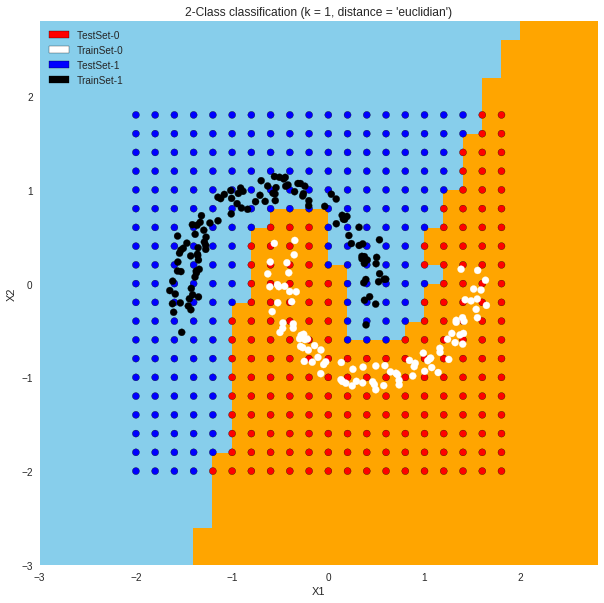
\includegraphics[width=0.7\textwidth]{q8_fig.png}  
	% reference folder/figure.pdf here and adjust width
	\captionsetup{labelformat=empty}
	\caption{}
	\label{fig:my_label}
\end{figure}


\item (To normalize, or not to normalize?)
Start from D2a.txt.  Perform 5-fold cross validation.
  \begin{enumerate}
  \item (5 pts) Do not normalize the data.  Report 1NN cross validation error rate for each fold, then the average (that's 6 numbers). 
  \item (5 pts) Normalize the data.  Report 1NN cross validation error rate (again 6 numbers).  (Hints: Do not normalize the labels!  The relevant quantities should be estimated from the training portion, but applied to both training and validation portions.  This should happen 5 times.  Also, you would either change $\x$ into $\tilde x = Lx$ but then use Euclidean distance on $\tilde x$, or do not change $x$ but use an appropriate $A$; don't mix the two.)
  \item (5 pts) Look at D2a.txt, explain the effect of normalization on CV error.  Hint: the first 4 features are different than the next 2 features.
  \end{enumerate}

\begin{soln}
	(a) The 5-fold Cross Validation Error Rates are: [0., 0., 0., 0., 0.]
	\newline
	Average error rate: 0.0
	
	(b) The 5-fold Cross Validation Error Rates for Normalized data: [0.07317073, 0.04878049, 0.125, 0.12820513, 0.1025641]
	\newline
	Average Error Rate: 0.09554409005628517
	
	(c) Picking up on the hint, if we look at the data, we notice that the first four features(or attributes) are essentially irrelevant.  We can prove this by running Cross-Validated 1NN predictions on three kinds of dataset: $X_{good}$ which has just the last two attributes. $X_{bad}$ which has the first four attributes. $X$ which is the original data.The average prediction error rates for training on the three different datasets pre and post-normalization are as follows:

	\begin{center}
	\begin{tabular}{ccc}\hline
		Training Dataset & CV-Error & CV Error-Normalized \\ \hline
		$X$ & 0.0 & 0.1 \\
		$X_{good}$ - only $x5$, $x6$ & 0.0 & 0.07\\
		$X_{bad} - x1,x2,x3,x4$ & 0.55 & 0.54\\ \hline
	\end{tabular}
	\end{center}


   Firstly, this is empirical proof that in the un-normalized dataset, the first four features are irrelevant and have no role at all in predicting labels of the test points. Secondly, since 1NN is essentially a distance-metric based classification method, the classification done using the distance based metric is heavily dominated by the last two features who have the maximum variance, and thus, impact the distance the most as the last two dimensions are analogous to being the Principal Components of the dataset. This significant difference in variance can be seen in the following table that is computed on the un-normalized data. 
    
    \begin{center}
    \begin{tabular}{ccccccc} \hline
    	Attributes & x1 & x2 & x3 & x4 & x5 & x6 \\ \hline
    	Variance & 0.000109 & 0.000113 & 0.000091 & 0.000095 & 0.863844 & 0.450556 \\ \hline
    \end{tabular}
	\end{center}

	However, after normalization is carried out, two things happen: 
	\begin{itemize}
		\item Due to rescaling of variance across all attributes to 1, the ompact of the last two features on the distance function is slightly diminished and noise is introduced which leads to an increase in error. 
		
		\item Due to change in variance across attributes, the covariance across the attributes also changes and thus, it might impact distance relations.
	\end{itemize} This fact can again be visually seen on a pairplot of the normalized data. The pairplot is able to retain geometrical properties of the original data but can give us an idea about the variation in range for all attributes. The range in the two relevant attributes is much greater than the other attributes in the unnormalized dataset, and so these relevant attributes play a greater role in the distance metric and is able to separate points better when compared to the normalized version where the range gets squished.

	\begin{figure}[h]
		\centering
		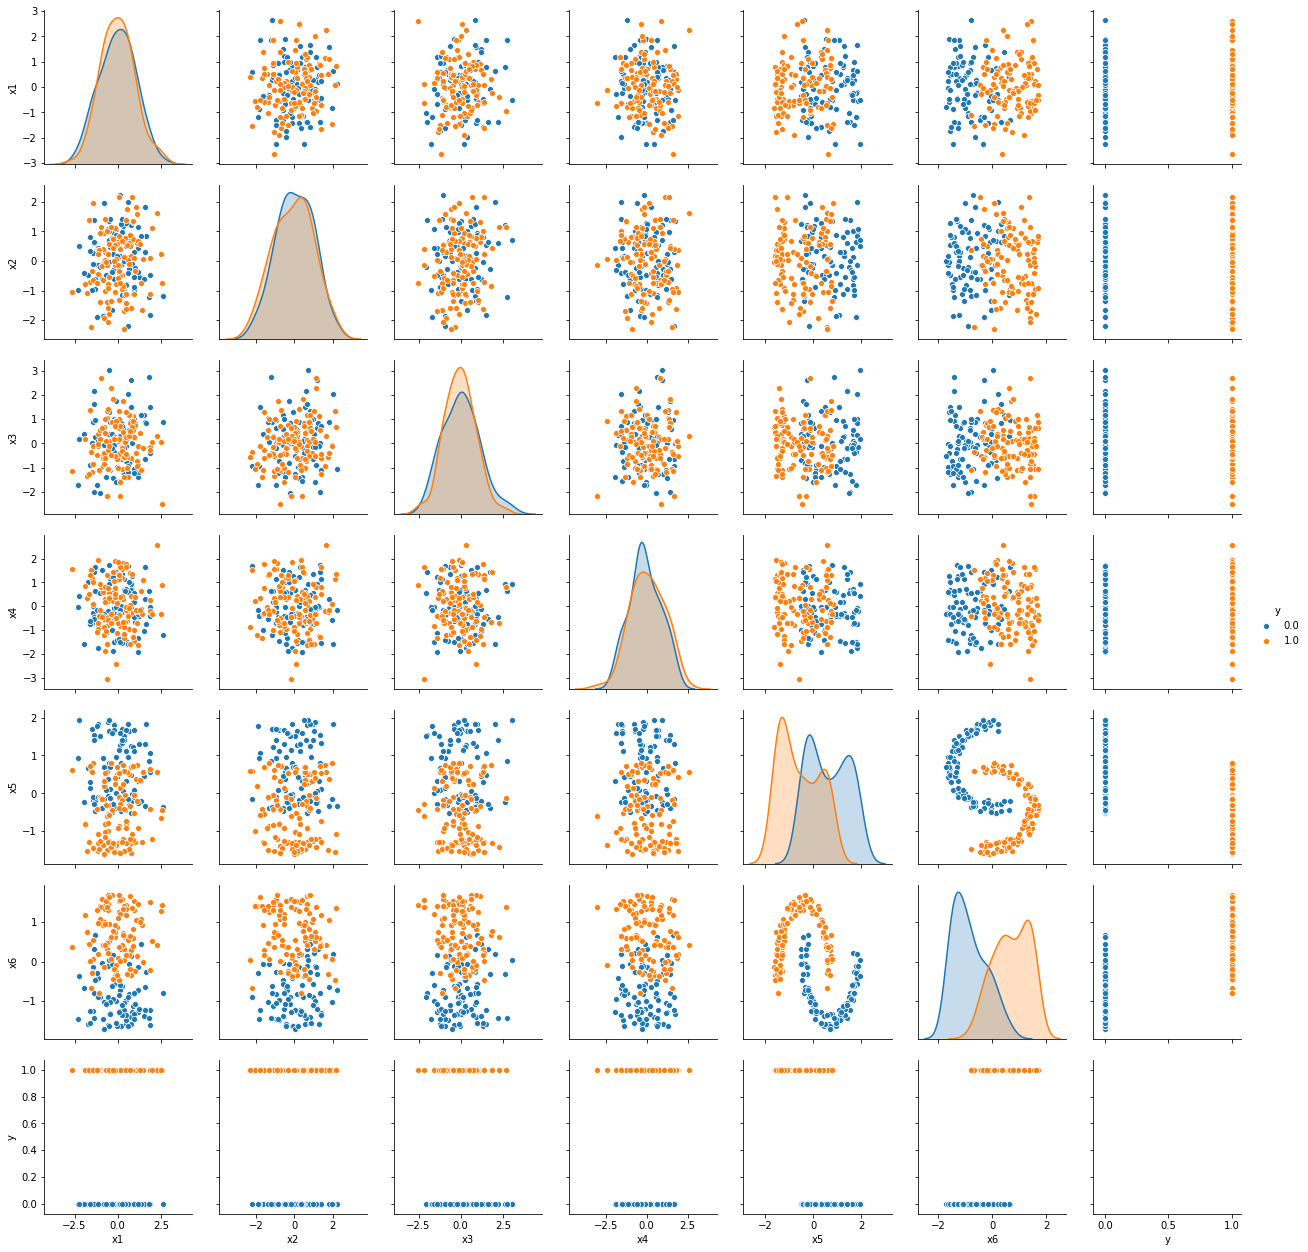
\includegraphics[width=0.55\textwidth]{q8_norm.png}  
		% reference folder/figure.pdf here and adjust width
		\captionsetup{labelformat=empty}
		\caption{}
		\label{fig:my_label}
	\end{figure}
		
	
    
\end{soln}

\item (Again.  10 pts)
Repeat the above question, starting from D2b.txt.

\begin{soln}
	(a) Unnormalized: The 5-fold Cross Validation Error Rates are: [0.15, 0.2, 0.15, 0.275, 0.2]
	\newline
	Average error rate: 0.195
	
	(b) Normalized: The 5-fold Cross Validation Error Rates are: [0.225, 0.1, 0.125, 0.15, 0.225]
	\newline
	Average error rate: 0.16
	
	(c) We can again look at the pairplots of the dataset pre-(plot 1) and post-(plot 2) normalization to see what's happening. 
	
	\begin{figure}[h]
		\centering
		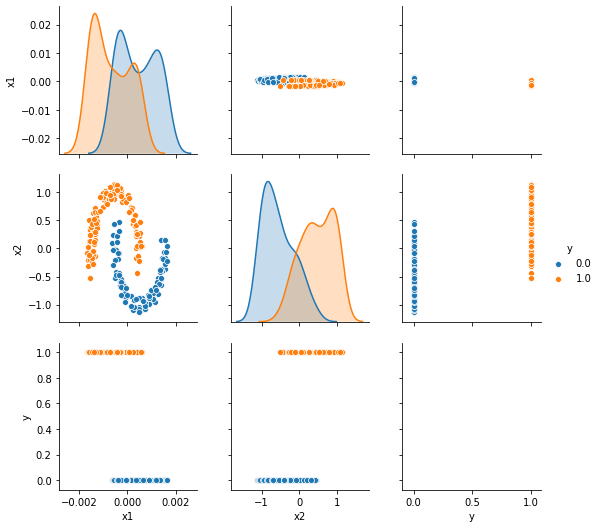
\includegraphics[width=0.55\textwidth]{q9_unnorm.png}  
		% reference folder/figure.pdf here and adjust width
		\captionsetup{labelformat=empty}
		\caption{}
		\label{fig:my_label}
	\end{figure}
	
	
	\begin{figure}[h]
		\centering
		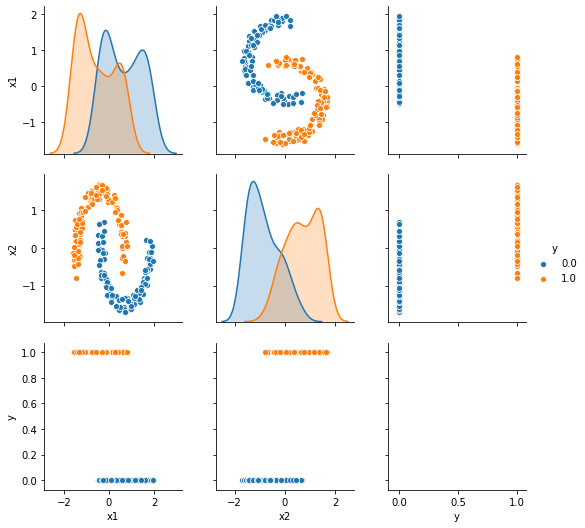
\includegraphics[width=0.55\textwidth]{q9_norm.png}  
		% reference folder/figure.pdf here and adjust width
		\captionsetup{labelformat=empty}
		\caption{}
		\label{fig:my_label}
	\end{figure}

	Looking at the pre-normalization plot, we can clearly see that feature x1 is quite irrelevant in its original form as its spread is not as big as x2, whereas in x2, the classes are distinctly separated and is the principal contributing factor in making the distance-based NN decisions. However, upon normalization, the constriction is removed and the attribute contributes meaningfully well to the classification decision being made that causes a small improvement in the CV test error.
	
\end{soln}

\item (5 pts) What do you learn from Q9 and Q10?

\begin{soln}
In distance based classification models like the 1NN, the decision is influenced by the measurement units also. When applying 1NN on multi-feature data, where the features have different ranges in their values, most of the distance based decisions will be made based on the features that have a larger range as this as across different samples, these are the dimensions along which there is the possibility of most variation. In the situation where most constricted(low-range) features are irrelevant(like in D2a), it doesn't make sense to normalize the data as that leads to dampening of the influence that the relevant features had on the distance based decision making. However, in cases where all attributes are more or less relevant(D2b), normalization can help improve the performance by rescaling one or more of the features. So, essentially, when the nearest neighbor decision is made on the basis of few the Principal components, it can really hurt to normalize if there are other irrelevant features in the dataset. 
\end{soln}


\item (Weka, 10 pts)
Repeat Q9 and Q10 with Weka.
Convert appropriate data files into ARFF format.
Choose classifiers / lazy / IBk.
Set $K=1$.
Choose 5-fold cross validation.
Let us know what else you needed to set.  Compare Weka's results to your Q9 and Q10.


\begin{soln}
	(I) D2a
	\newline
	    (i) The CV-error for unnormalized data: 0.05 
	    \newline
 		(ii) The CV error for normalized data: 0.05
 		
	(II) D2b
	\newline 
		(i) The CV-error for unnormalized data: 0
		\newline 
		(ii) The CV error for normalized data: 0
	
\end{soln}

\end{enumerate}

\bibliographystyle{apalike}
\end{document}
